% Provenance (never printed): old terminale S material on past climates (ice cores,
% pollen, ocean sediments and oxygen isotopes, glacial-interglacial cycles, the
% astronomical rhythm told, climates of deep time), read from data. Owner (Sync 0/1):
% climate archive and proxy, ice core, glacial period, interglacial and glacial cycle,
% pollen analysis, Last Glacial Maximum. Recalled: glacier, ice sheet, ice age (Book 1,
% grade 8); the first look at the ice-core records (Book 1, grade 9); isotopes
% (physics); greenhouse gases (chemistry); the time scale (Book 1, grade 7). The
% delta notation of isotopes is Book 3's: isotope curves are read here as told,
% without a definition. The orbital theory of climate belongs to a university book:
% told here only. Physical science only, in the IPCC's calibrated words.
% Figures: figdata/grade-12/ice_age_records.py (tests/grade-12/test_ice_age_records.py).
\chapter{Ler os climas do passado}\label{ch:g12:past-climates}

Em Dome~C, a \qty{3233}{m} de altitude sobre o manto de gelo da Antártida
Oriental, o ar tem em média cerca de \qty{-55}{\degreeCelsius} ao longo do
ano. Uma sonda que trabalhou ali parou a uma profundidade de \qty{3260}{m},
cerca de \qty{15}{m} acima da rocha sob o gelo. O gelo mais profundo que ela
trouxe contém bolhas minúsculas de ar de uns \num{800000} anos: uma amostra
da atmosfera de muito antes dos primeiros agricultores. Este capítulo
lê o clima do passado no gelo, na lama dos lagos e do fundo do oceano, e
nas rochas, e pergunta o que ele diz sobre hoje.
% ledger: ipev:concordia, edc3:drilling, jouzel07:edc

\begin{omfigure}
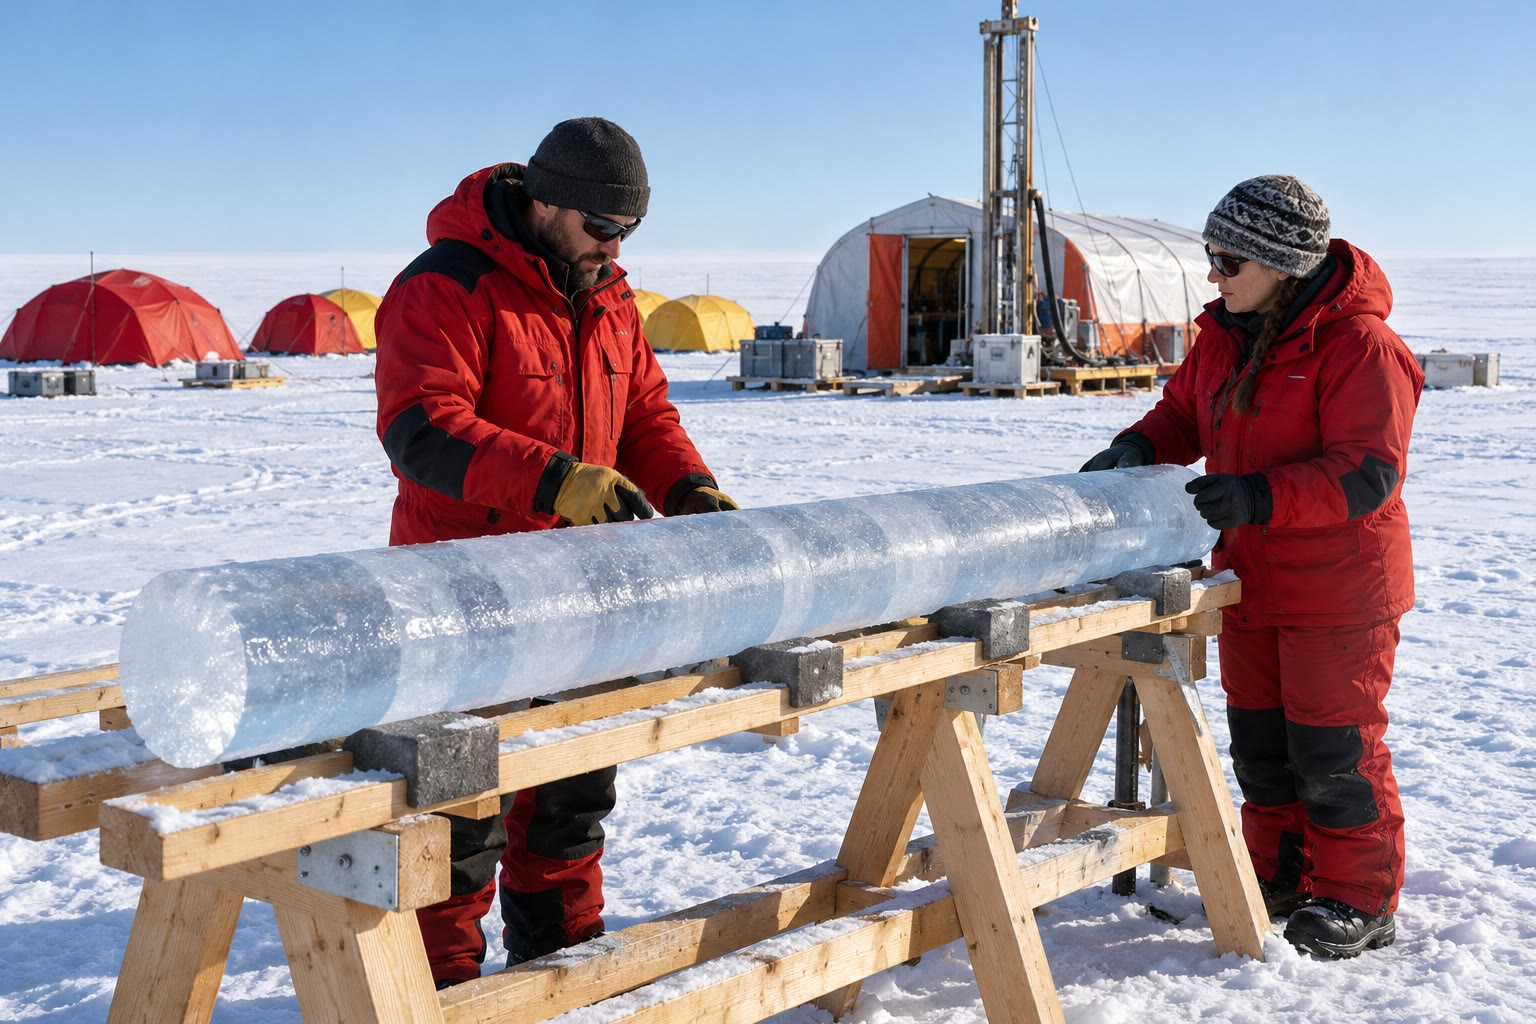
\includegraphics[width=0.56\linewidth]{images/book2/ai/g12-ice-coring-camp.jpg}

{\small Um acampamento de perfuração de gelo num manto de gelo polar: a
sonda trabalha sob a torre e o abrigo, e cada trecho de testemunho é
estendido, registrado e embalado antes de viajar para o laboratório.
Ilustração gerada por IA.}
\end{omfigure}

\begin{recall}
Uma geleira é uma massa de gelo que dura de um ano para o outro e flui sob o
seu próprio peso; um manto de gelo cobre uma grande parte de um continente;
uma glaciação é um longo período frio em que os mantos de gelo se estendem
muito além dos polos (Livro 1, 8º ano). Nos \omterm{def:g12:past-climates:ice-core}{testemunhos de gelo} da
Antártida, a neve registra a temperatura do ar e as bolhas guardam o próprio
ar, e os dois registros sobem e descem juntos (Livro 1, 9º ano). Os átomos
de um mesmo elemento podem diferir pelo seu número de nêutrons: esses
isótopos se comportam da mesma forma na química, mas diferem na massa (os
livros de física). O gás carbônico é um gás de efeito estufa (os livros de
química). O período Quaternário começou há 2.58 milhões de anos
(Livro 1, 7º ano).
\end{recall}
% ledger: ics:base.Quaternary (shared), nasaeo:o18 (snow poor in heavy isotopes)

\section{Arquivos e indicadores}

Ninguém mediu a temperatura do ar há \num{20000} anos. Mas a Terra guardou
registros sem querer: camadas de gelo e de lama, conchas e troncos de
árvores, cada um dos quais mudou com o clima em que se formou.

\begin{definition}[Arquivo climático; indicador indireto]\label{def:g12:past-climates:proxy}
Um \emph{arquivo climático}\index{arquivo climatico@arquivo climático} é um
material natural depositado em camadas, uma depois da outra, que guarda um
vestígio do clima da época em que se formou: o gelo polar, os sedimentos dos
lagos e do fundo do oceano, os anéis das árvores, os corais, os depósitos
das cavernas. Um \emph{indicador indireto}\index{indicador indireto}
(em inglês, \textit{proxy}) é uma grandeza medida num arquivo que substitui
uma variável climática que não foi medida: a parte de isótopos pesados na
neve antiga para a temperatura do ar, a parte de cada tipo de pólen na lama
dos lagos para a vegetação e, portanto, para o clima.
\end{definition}
% ledger: ncei:proxy, ncei:pollen, nasaeo:o18

\begin{center}
\small
\begin{tabular}{|l|l|l|}
\hline
\textbf{arquivo} & \textbf{\omterm{def:g12:past-climates:proxy}{indicador}} & \textbf{informa sobre} \\
\hline
gelo polar & isótopos pesados do gelo & temperatura do ar sobre o gelo \\
 & ar das bolhas & gás carbônico, metano \\
sedimentos de lagos, turfa & pólen & vegetação, depois clima \\
sedimentos oceânicos & oxigênio-18 das conchas & volume de gelo, temperatura do fundo \\
anéis das árvores & largura dos anéis & condições de crescimento, ano a ano \\
corais, depósitos de cavernas & isótopos, faixas de crescimento & temperatura (mar, ar), chuva \\
\hline
\end{tabular}

\medskip
{\small Os principais \omterm{def:g12:past-climates:proxy}{arquivos climáticos} e alguns dos seus \omterm{def:g12:past-climates:proxy}{indicadores}.}
\end{center}
% ledger: ncei:proxy, nasaeo:o18

Todo \omterm{def:g12:past-climates:proxy}{indicador} precisa de duas coisas antes de poder ser lido. Ele precisa
de um \emph{relógio}: a idade de cada camada, pela contagem das camadas
anuais onde elas são visíveis, pela datação radiométrica
(\cref{ch:g12:age-of-the-earth}), ou pela correlação do registro com outro
já datado. E ele precisa de uma \emph{calibração}: a relação entre o que é
medido e a variável climática, estabelecida hoje, quando as duas podem ser
medidas juntas.

\begin{method}[Ler um registro de indicador]
\begin{enumerate}
  \item Identifique o arquivo e o \omterm{def:g12:past-climates:proxy}{indicador}: o que foi medido, e em quê?
  \item Descubra em que sentido o tempo corre no eixo, e em que unidade;
        verifique se o eixo do \omterm{def:g12:past-climates:proxy}{indicador} está invertido.
  \item Traduza o \omterm{def:g12:past-climates:proxy}{indicador}: um valor mais alto significa mais quente ou
        mais frio, mais gelo ou menos?
  \item Observe o espaçamento das amostras: um registro cujos pontos estão a
        \num{2000} anos de distância não pode mostrar uma mudança que durou
        um século.
  \item Leia os valores nas datas pedidas, ou as médias num intervalo, e
        calcule as variações e as taxas.
  \item Diga o que o registro mostra no seu local, e só então se ele vale
        para a Terra inteira.
\end{enumerate}
\end{method}

\section{Testemunhos de gelo}

\begin{definition}[Testemunho de gelo]\label{def:g12:past-climates:ice-core}
Um \emph{testemunho de gelo}\index{testemunho de gelo} é um cilindro de gelo
extraído por perfuração de um manto de gelo ou de uma geleira. A sua
profundidade dá a idade do gelo, mais antigo quanto mais profundo; o gelo
registra a temperatura do ar em que a sua neve caiu, e as suas bolhas
guardam amostras do ar da época.
\end{definition}
% ledger: ncei:proxy, jouzel07:edc

A neve fresca é sobretudo ar. Enterrada sob a neve dos anos seguintes, ela
é comprimida em \emph{firn}, uma neve compactada cujos poros ainda deixam o
ar passar. A uma densidade de cerca de 820 a \qty{830}{kg/m^3}, alcançada a
50 a \qty{120}{m} de profundidade, os poros se fecham e o ar fica preso em bolhas. O gelo guarda, portanto, dois
registros diferentes. O ar das bolhas é uma amostra da atmosfera, cujo gás
carbônico e cujo metano são medidos no laboratório. O próprio gelo guarda a
temperatura: as moléculas de água que contêm um isótopo pesado (deutério ou
oxigênio-18) se condensam mais facilmente que as leves, então, quanto mais
frio o ar no caminho até o polo, mais pobre em isótopos pesados fica a neve.
% ledger: firn:close-off, nasaeo:o18

\begin{omfigure}
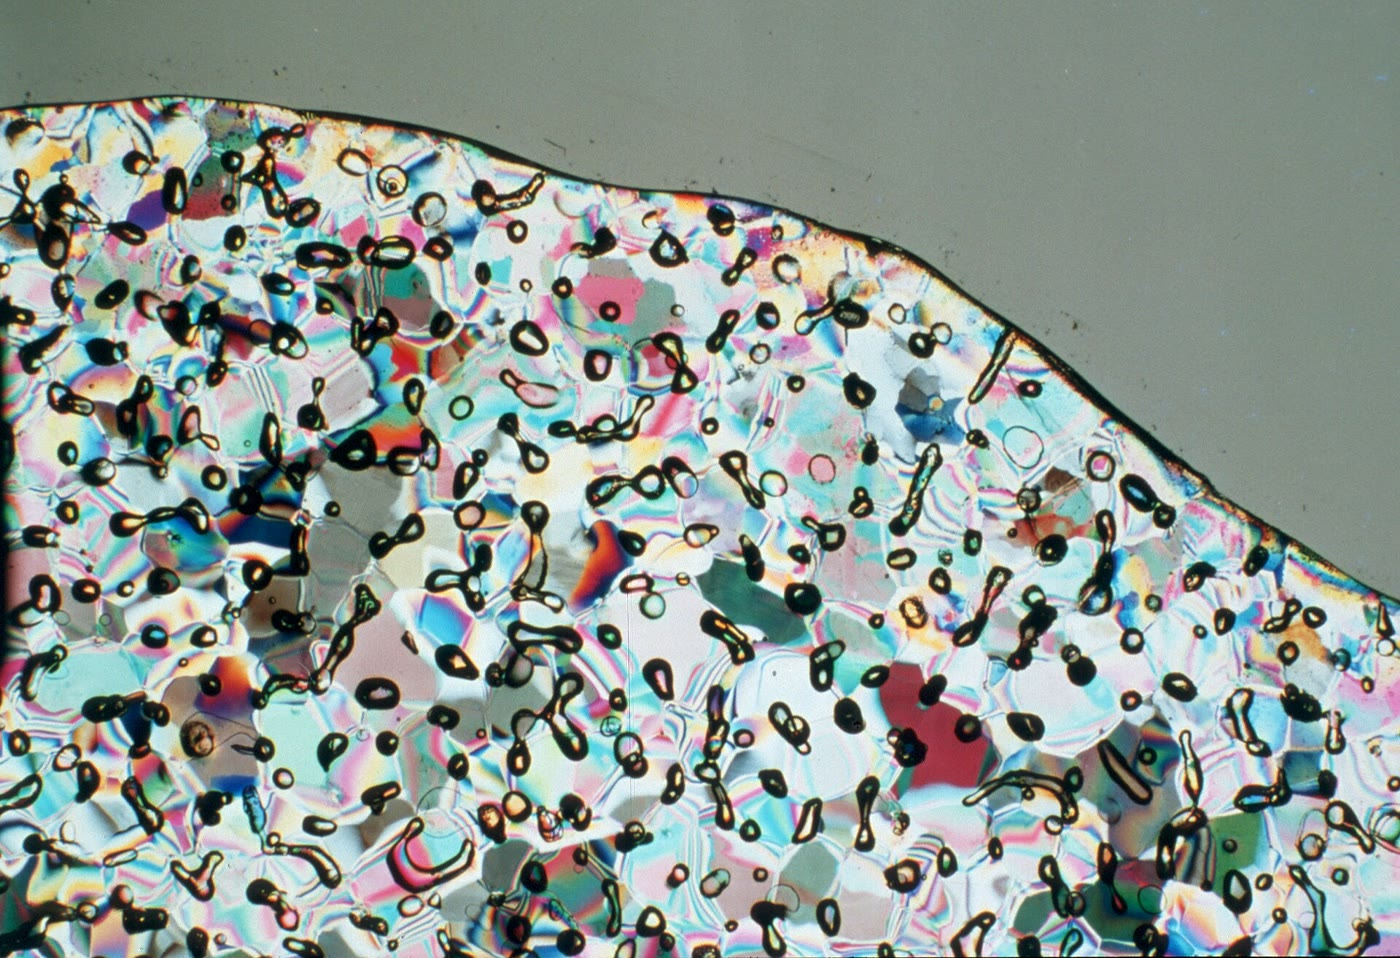
\includegraphics[width=0.50\linewidth]{images/book2/g12-ice-bubbles.jpg}

{\small Uma lâmina de gelo antártico vista sob luz polarizada, que colore
os cristais de gelo: os pontos escuros são bolhas de ar preso. Fotografia
CSIRO Atmospheric Research, CC~BY~3.0 (Wikimedia Commons).}
\end{omfigure}
% ledger: photo:g12-ice-bubbles

O deutério do testemunho de Dome~C foi convertido numa temperatura sobre o
gelo, dada como uma variação em relação à média dos últimos mil anos. O gás
carbônico vem das bolhas de vários testemunhos antárticos, reunidos num só
registro. Os dois estão representados abaixo sobre um mesmo eixo do tempo.

\begin{omfigure}
\begin{tikzpicture}
\begin{axis}[omrecord, scale only axis, width=0.74\linewidth, height=4.8cm,
  xmin=0, xmax=800, x dir=reverse, ymin=-12, ymax=8, axis y line*=left,
  xtick={0,100,...,800}, ytick={-10,-5,0,5},
  xlabel={milhares de anos antes de 1950},
  ylabel={variação de temperatura (\unit{\degreeCelsius})}]
% data:edc-jouzel, 2-kyr means (figdata/grade-12/ice_age_records.py)
\addplot[omWarm, line width=0.7pt] table[x=age_kyr, y=temp_C] {figdata/out/grade-12-ice_age_records-edc.dat};
\end{axis}
\begin{axis}[scale only axis, width=0.74\linewidth, height=4.8cm,
  xmin=0, xmax=800, x dir=reverse, ymin=60, ymax=320, axis y line*=right,
  axis x line=none, ytick={180,220,260,300}, ylabel={gás carbônico (ppm)},
  every axis label/.append style={font=\small}, tick label style={font=\small}]
% data:co2-bereiter, 2-kyr means
\addplot[black, line width=0.7pt] table[x=age_kyr, y=co2_ppm] {figdata/out/grade-12-ice_age_records-co2.dat};
\coordinate (lt) at (axis cs:560,70);
\coordinate (lc) at (axis cs:560,312);
\end{axis}
\node[font=\scriptsize, text=omWarm, anchor=south] at (lt) {temperatura em Dome~C (escala à esquerda)};
\node[font=\scriptsize, anchor=north] at (lc) {gás carbônico (escala à direita)};
\end{tikzpicture}

{\small Oitocentos mil anos de gelo antártico, em médias por intervalos de
\num{2000} anos. Em vermelho: a temperatura em Dome~C em relação aos últimos
mil anos (Jouzel e colaboradores, 2007); em preto: o gás carbônico das
bolhas (Bereiter e colaboradores, 2015). Hoje está à direita.}
\end{omfigure}
% ledger: data:edc-jouzel, data:co2-bereiter

As duas curvas compartilham um mesmo padrão: um deslizamento lento e
irregular para o frio ao longo de dezenas de milhares de anos, depois uma
subida rápida de volta ao calor, depois de novo o deslizamento.

\begin{definition}[Período glacial; interglacial; ciclo glacial]\label{def:g12:past-climates:glacial-cycle}
Um \emph{período glacial}\index{periodo glacial@período glacial} é um
intervalo frio dentro de uma glaciação, durante o qual os mantos de gelo
crescem muito além do seu tamanho atual. Um
\emph{interglacial}\index{interglacial} é um intervalo quente entre dois
períodos glaciais, com mantos de gelo próximos dos de hoje ou menores; nós
vivemos num, que começou há cerca de \num{11000} anos. Um \emph{ciclo
glacial}\index{ciclo glacial} é um período glacial com o interglacial que
o encerra.
\end{definition}
% ledger: ipcc:ref-periods (LDT ends 11 ka); the count of cycles is read from the figure (data:edc-jouzel)

Ao longo de todo o registro, a temperatura em Dome~C vai de
\qty{-10.6}{\degreeCelsius}, há cerca de \num{24000} anos, a
\qty{+5.5}{\degreeCelsius}, há cerca de \num{129000} anos; o gás carbônico,
de \qty{174}{ppm} a \qty{299}{ppm}. A figura, em médias por intervalos de
\num{2000} anos, suaviza um pouco esses extremos. A contagem dos picos
quentes dá oito ou nove \omterm{def:g12:past-climates:glacial-cycle}{ciclos glaciais}, e o ritmo mais forte do registro de
temperatura, calculado a partir dos seus dados, tem um período de cerca de
\num{98000} anos.
% ledger: data:edc-jouzel, data:co2-bereiter (ice_age_records.py: edc_min_C -10.58 at 24.0 kyr, edc_max_C 5.46 at 128.7 kyr, co2 173.71 and 298.6, edc_period_kyr 97.5)

\begin{proposition}[Temperatura e gás carbônico variam juntos]\label{prop:g12:past-climates:correlation}
% ledger: data:edc-jouzel, data:co2-bereiter (ice_age_records.py: r_temp_co2 0.9165, fit 266.57 + 7.827 T, 1639 pairs)
Ao longo dos últimos \num{800000} anos, a temperatura antártica e o gás
carbônico do ar variaram juntos. Associar cada uma das 1639 medições de gás
carbônico com mais de \num{2000} anos à temperatura de Dome~C da mesma idade
dá um coeficiente de correlação $r = 0.92$, e a
reta de mínimos quadrados
\[
  \mathrm{CO_2} \approx \qty{267}{ppm} + \qty{7.8}{ppm/\degreeCelsius} \times \Delta T ,
\]
em que $\Delta T$ é a variação de temperatura em Dome~C.
\end{proposition}

\begin{proof}[Como é calculado]
Para cada amostra de gás carbônico, a temperatura na sua idade é lida no
registro de Dome~C por interpolação entre os dois pontos de temperatura mais
próximos. O coeficiente de correlação dos 1639 pares, um número entre $-1$ e
$1$ que mede quão perto os pontos ficam de uma reta (os livros de
matemática), é calculado junto com a reta de mínimos quadrados; os dois são
calculados no script da figura e verificados pelo seu teste.
\end{proof}

\begin{omfigure}
\begin{tikzpicture}
\begin{axis}[omrecord, width=0.70\linewidth, height=5.2cm, xmin=-12, xmax=6,
  ymin=160, ymax=310, xlabel={variação de temperatura em Dome~C (\unit{\degreeCelsius})},
  ylabel={gás carbônico (ppm)}]
% data:edc-jouzel, data:co2-bereiter (pairs and fit in ice_age_records.py)
\addplot[only marks, mark=*, mark size=0.6pt, omDef, opacity=0.45] table[x=temp_C, y=co2_ppm] {figdata/out/grade-12-ice_age_records-pairs.dat};
\addplot[omThm, line width=1pt] table[x=temp_C, y=co2_ppm] {figdata/out/grade-12-ice_age_records-fit.dat};
\node[font=\scriptsize, text=omThm, anchor=south east, fill=white, inner sep=1pt] at (axis cs:-1.5,295) {reta de mínimos quadrados, $r = 0.92$};
\end{axis}
\end{tikzpicture}

{\small Cada ponto é uma medição de gás carbônico do gelo antártico,
colocada na temperatura de Dome~C da mesma idade: as épocas frias tinham
pouco gás carbônico, as épocas quentes muito mais. Calculado a partir de
Jouzel e colaboradores (2007) e de Bereiter e colaboradores (2015).}
\end{omfigure}

Uma correlação não diz qual mudou primeiro, nem se uma terceira causa moveu
os dois: o coeficiente seria o mesmo se a temperatura comandasse o gás
carbônico, se o gás carbônico comandasse a temperatura, ou se cada um
empurrasse o outro. O que dá o ritmo de cerca de \num{100000} anos é contado
na seção sobre o oceano, mais abaixo, e como o gás carbônico age sobre a
temperatura, no \cref{ch:g12:climate-change}.

\subsection{O Último Máximo Glacial}

\begin{definition}[Último Máximo Glacial]\label{def:g12:past-climates:lgm}
O \emph{Último Máximo Glacial}\index{Ultimo Maximo Glacial@Último Máximo Glacial} é a época, de cerca de
\num{23000} a \num{19000} anos atrás, em que os mantos de gelo do último
\omterm{def:g12:past-climates:glacial-cycle}{período glacial} estavam no seu maior tamanho.
\end{definition}
% ledger: ipcc:ref-periods

No \omterm{def:g12:past-climates:lgm}{Último Máximo Glacial}, mantos de gelo cobriam boa parte da América do
Norte e do noroeste da Eurásia, e o clima era mais seco e mais poeirento que
hoje. As avaliações estimam que a temperatura global da superfície era de
\qty{5}{\degreeCelsius} a \qty{7}{\degreeCelsius} mais baixa que em 1850--1900
(\emph{média confiança}), com o gás carbônico entre 188 e \qty{194}{ppm}.
A água presa nos mantos de gelo veio do oceano: o nível médio global do mar
estava 125 a \qty{134}{m} abaixo do de hoje.
% ledger: ipcc:ref-periods, ipcc:lgm-cooling, ipcc:fig2-34, ipcc:lgm-sea, lambeck14:lgm

Um mar mais baixo descobre o fundo raso em volta dos continentes. O mapa
abaixo baixa o mar em \qty{130}{m}, o meio dessa faixa, sobre o fundo do
Sudeste Asiático tal como ele é hoje.

\begin{omfigure}
\begin{tikzpicture}
\begin{axis}[omrecord, axis equal image, width=0.62\linewidth, xmin=92, xmax=122,
  ymin=-11, ymax=24, grid=none, axis x line=box, axis y line=box,
  xtick={95,105,115}, ytick={-10,-5,...,20},
  xticklabel={\pgfmathprintnumber{\tick}\textdegree L},
  yticklabels={10\textdegree S, 5\textdegree S, 0\textdegree, 5\textdegree N, 10\textdegree N, 15\textdegree N, 20\textdegree N}]
% data:b2-etopo-sunda (raster computed in ice_age_records.py; sea level lowered by 130 m)
\addplot graphics[xmin=91.95, xmax=122.05, ymin=-11.05, ymax=24.05] {figdata/out/grade-12-ice_age_records-sunda.png};
\node[font=\scriptsize] at (axis cs:114.5,0.5) {Bornéu};
\node[font=\scriptsize, rotate=-45] at (axis cs:101.9,-1.3) {Sumatra};
\node[font=\scriptsize] at (axis cs:110.5,-8.6) {Java};
\node[font=\scriptsize, rotate=-60] at (axis cs:102.2,4.0) {Pen. Malaia};
\node[font=\scriptsize] at (axis cs:103,16.5) {Indochina};
\node[font=\scriptsize, align=center] at (axis cs:106.5,3.5) {Plataforma\\de\\Sunda};
\node[font=\scriptsize, align=center] at (axis cs:114.5,13) {Mar da China\\Meridional};
\node[font=\scriptsize, align=center] at (axis cs:96,-6) {Oceano\\Índico};
\end{axis}
\end{tikzpicture}

{\small O Sudeste Asiático com o mar \qty{130}{m} mais baixo que hoje. Em
verde: as terras de hoje; em bege: o fundo que um nível do mar \qty{130}{m}
mais baixo descobre; em azul: o mar. O relevo atual é usado, então a linha
de costa é só aproximada. Calculado a partir do relevo ETOPO1 (NOAA), a
cada 0.1 grau.}
\end{omfigure}
% ledger: data:b2-etopo-sunda, ipcc:lgm-sea

Bornéu, Sumatra e Java formam uma só terra com a Península Malaia e a
Indochina: a Plataforma de Sunda, hoje sob um mar raso, era terra firme. No mapa, uma
descida de apenas cerca de \qty{36}{m} basta para ligar Bornéu à Ásia, e
Sumatra e Java se ligam a ela antes. No mapa,
as terras acima do mar passam de 4.11 a 7.16 milhões de quilômetros
quadrados, 1.74 vez mais. Na Terra inteira, a mesma descida de \qty{130}{m}
eleva a parte da superfície acima do mar de \qty{29.0}{\percent} a
\qty{33.5}{\percent}, cerca de 23 milhões de quilômetros quadrados de terras
novas.
% ledger: data:b2-etopo-sunda, data:etopo1 (ice_age_records.py: borneo_link_m -36; sunda_land_now_km2 4.105e6, lgm 7.161e6, ratio 1.744; world_land_now_frac 0.2904, lgm 0.3352, world_gain_km2 2.285e7)

\begin{example}[A última deglaciação]
O aquecimento que se seguiu ao \omterm{def:g12:past-climates:lgm}{Último Máximo Glacial} é chamado de última
transição deglacial; as avaliações a situam entre cerca de \num{18000} e
\num{11000} anos atrás. No registro de Dome~C, a temperatura média do
\omterm{def:g12:past-climates:lgm}{Último Máximo Glacial} (de \num{23000} a \num{19000} anos atrás) é de
\qty{-9.4}{\degreeCelsius}; a média do intervalo seguinte, de \num{11000} a
\num{9000} anos atrás, é de \qty{-0.4}{\degreeCelsius}. O ar sobre a
Antártida se aqueceu \qty{9.0}{\degreeCelsius}, enquanto o seu gás
carbônico subia de \qty{190}{ppm} a \qty{264}{ppm}, ou seja, \qty{74}{ppm}.
Na Terra inteira, o aquecimento foi o resfriamento avaliado de 5 a
\qty{7}{\degreeCelsius}, cerca de \qty{6}{\degreeCelsius}, distribuído pelos
\num{7000} anos da transição:
\[
  \frac{\qty{6}{\degreeCelsius}}{\num{7000}\ \text{anos}} \approx
  \qty{0.86}{\degreeCelsius} \text{ por mil anos.}
\]
Nesse meio-tempo, o nível do mar subiu de cerca de \qty{-120}{m} a
\qty{-50}{m}, em média cerca de \qty{10}{mm} por ano.
\end{example}
% ledger: ipcc:ref-periods, ipcc:lgm-cooling, ipcc:lgm-sea, data:edc-jouzel, data:co2-bereiter (ice_age_records.py: edc_lgm_C -9.389, edc_holo_C -0.360, rise 9.029; co2 189.67, 264.10, rise 74.43; ldt_mean_rate 0.857)

\begin{omfigure}
\begin{tikzpicture}
\begin{axis}[omrecord, scale only axis, width=0.74\linewidth, height=4.6cm,
  xmin=0, xmax=30, x dir=reverse, ymin=-11, ymax=12, axis y line*=left,
  xtick={0,5,...,30}, ytick={-10,-5,0},
  xlabel={milhares de anos antes de 1950},
  ylabel={variação de temperatura (\unit{\degreeCelsius})}]
\fill[omDef!10] (axis cs:23,-11) rectangle (axis cs:19,12);
\fill[omProp!12] (axis cs:18,-11) rectangle (axis cs:11,12);
% data:edc-jouzel, every sample
\addplot[omWarm, line width=0.6pt] table[x=age_kyr, y=temp_C] {figdata/out/grade-12-ice_age_records-edc30.dat};
\coordinate (lgm) at (axis cs:21,11.6);
\coordinate (ldt) at (axis cs:14.5,11.6);
\coordinate (lt) at (axis cs:5.5,-3.6);
\end{axis}
\begin{axis}[scale only axis, width=0.74\linewidth, height=4.6cm,
  xmin=0, xmax=30, x dir=reverse, ymin=60, ymax=290, axis y line*=right,
  axis x line=none, ytick={200,240,280}, ylabel={gás carbônico (ppm)},
  every axis label/.append style={font=\small}, tick label style={font=\small}]
% data:co2-bereiter, every sample
\addplot[black, line width=0.6pt, mark=*, mark size=0.5pt] table[x=age_kyr, y=co2_ppm] {figdata/out/grade-12-ice_age_records-co230.dat};
\coordinate (lc) at (axis cs:26.5,196);
\end{axis}
\node[font=\scriptsize, anchor=north, align=center] at (lgm) {Último Máximo\\Glacial};
\node[font=\scriptsize, anchor=north, align=center] at (ldt) {última transição\\deglacial};
\node[font=\scriptsize, text=omWarm, anchor=north] at (lt) {temperatura (à esquerda)};
\node[font=\scriptsize, anchor=south] at (lc) {\shortstack{gás carbônico\\(à direita)}};
\end{tikzpicture}

{\small Os últimos \num{30000} anos em Dome~C, todas as medições: a
temperatura (em vermelho) e o gás carbônico (em preto) sobem juntos ao sair
do \omterm{def:g12:past-climates:lgm}{Último Máximo Glacial}. Sombreados: o \omterm{def:g12:past-climates:lgm}{Último Máximo Glacial} e a última
transição deglacial, tal como o IPCC os data. Dados: Jouzel e colaboradores
(2007), Bereiter e colaboradores (2015).}
\end{omfigure}
% ledger: data:edc-jouzel, data:co2-bereiter, ipcc:ref-periods

\section{O pólen}

Toda primavera, as plantas liberam nuvens de pólen. A maior parte dele se
perde, mas uma parte cai sobre lagos e turfeiras, afunda e é enterrada na
lama, onde guarda um registro da vegetação que crescia em volta. E os grãos
de cada tipo de planta têm a sua própria forma e o seu próprio tamanho.
% ledger: ncei:pollen

\begin{omfigure}
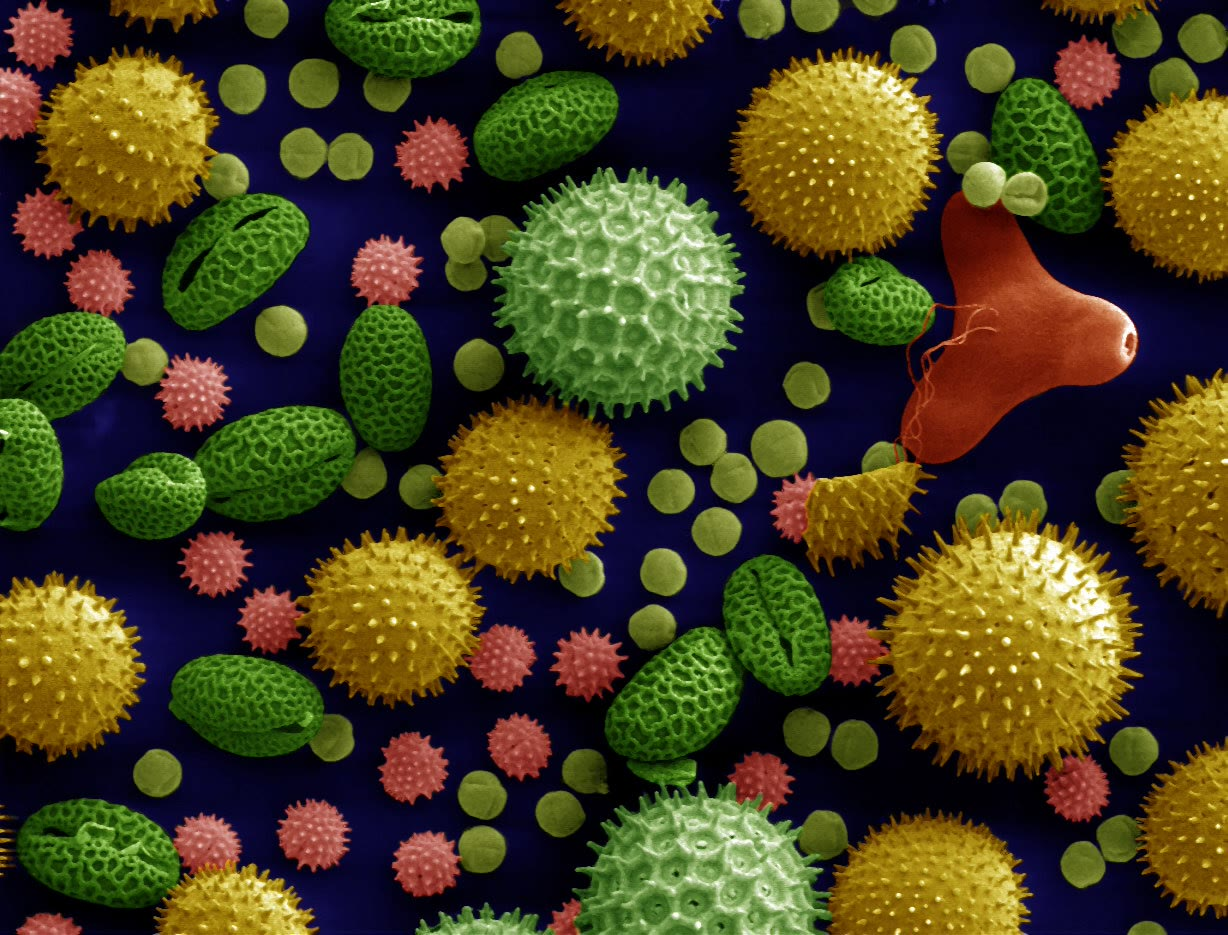
\includegraphics[width=0.46\linewidth]{images/book2/g12-pollen-sem.jpg}

{\small Grãos de pólen de cinco plantas comuns (girassol, ipomeia,
malva-rosa, lírio e prímula) vistos com um microscópio eletrônico de
varredura, em falsas cores. Cada tipo de planta tem a sua própria forma de
grão. Dartmouth Electron Microscope Facility (domínio público, via Wikimedia
Commons).}
\end{omfigure}
% ledger: photo:g12-pollen

\begin{definition}[Análise polínica]\label{def:g12:past-climates:pollen}
A \emph{análise polínica}\index{analise polinica@análise polínica} é a
leitura da vegetação do passado a partir do pólen conservado nos
sedimentos: em cada camada de um testemunho, os grãos são identificados e
contados, e a parte de cada tipo de planta, em porcentagem dos grãos
contados, é representada em função da profundidade num \emph{diagrama
polínico}\index{diagrama polinico@diagrama polínico}.
\end{definition}
% ledger: ncei:pollen

A contagem do pólen desse modo começou com o geólogo sueco Lennart von
Post, que apresentou o primeiro \omterm{def:g12:past-climates:pollen}{diagrama polínico} moderno, com números, em
1916; um diagrama assim mostra a profundidade descendo na página e uma curva
para cada tipo de planta. A vegetação, por sua vez, fala do clima: gramíneas
e outras ervas quase sem árvores significam uma paisagem aberta e fria,
enquanto o carvalho e a aveleira precisam de verões quentes.
% ledger: rull18:von-post; the Varden diagram is invented (ice_age_records.py POLLEN)

\begin{omfigure}
\begin{tikzpicture}
\pgfplotsset{pollen/.style={scale only axis, height=6cm, ymin=300, ymax=600,
  y dir=reverse, xmin=0, axis x line*=bottom, axis y line*=left, axis line style={-},
  tick label style={font=\scriptsize}, title style={font=\small, yshift=-4pt, text depth=0.25ex, text height=1.6ex},
  ytick={300,350,...,600}, xmajorgrids, ymajorgrids,
  grid style={gray!22, line width=0.3pt}}}
\begin{axis}[pollen, name=p1, width=3.0cm, xmax=100, xtick={0,20,...,80}, title={ervas},
  ylabel={profundidade (cm)}, every axis label/.append style={font=\small}]
\addplot[fill=omLithSand, draw=black!70, line width=0.4pt] table[x=pct, y=depth_cm] {figdata/out/grade-12-ice_age_records-pol-herbs.dat};
\coordinate (z1) at (axis cs:0,550);
\coordinate (z2) at (axis cs:0,470);
\coordinate (z3) at (axis cs:0,425);
\end{axis}
\begin{axis}[pollen, name=p2, at={(p1.south east)}, anchor=south west, xshift=0.3cm,
  width=1.8cm, xmax=60, xtick={0,20,40}, title={bétula}, yticklabels={}]
\addplot[fill=omHypsLandB, draw=black!70, line width=0.4pt] table[x=pct, y=depth_cm] {figdata/out/grade-12-ice_age_records-pol-birch.dat};
\end{axis}
\begin{axis}[pollen, name=p3, at={(p2.south east)}, anchor=south west, xshift=0.3cm,
  width=1.8cm, xmax=60, xtick={0,20,40}, title={pinheiro}, yticklabels={}]
\addplot[fill=omHypsLandA, draw=black!70, line width=0.4pt] table[x=pct, y=depth_cm] {figdata/out/grade-12-ice_age_records-pol-pine.dat};
\end{axis}
\begin{axis}[pollen, name=p4, at={(p3.south east)}, anchor=south west, xshift=0.3cm,
  width=1.2cm, xmax=40, xtick={0,20}, title={aveleira}, yticklabels={}]
\addplot[fill=omHypsLandD, draw=black!70, line width=0.4pt] table[x=pct, y=depth_cm] {figdata/out/grade-12-ice_age_records-pol-hazel.dat};
\end{axis}
\begin{axis}[pollen, name=p5, at={(p4.south east)}, anchor=south west, xshift=0.3cm,
  width=1.5cm, xmax=50, xtick={0,20,40}, title={carvalho}, yticklabels={}]
\addplot[fill=omHypsLandE, draw=black!70, line width=0.4pt] table[x=pct, y=depth_cm] {figdata/out/grade-12-ice_age_records-pol-oak.dat};
\coordinate (e1) at (axis cs:50,550);
\coordinate (e2) at (axis cs:50,470);
\coordinate (e3) at (axis cs:50,425);
\coordinate (top) at (axis cs:50,300);
\coordinate (bot) at (axis cs:50,600);
\end{axis}
\draw[densely dashed, black!70] (z1) -- (e1 -| p5.east);
\draw[densely dashed, black!70] (z2) -- (e2 -| p5.east);
\draw[densely dashed, black!70] (z3) -- (e3 -| p5.east);
\node[font=\scriptsize, anchor=west] at ($(bot -| p5.east)!0.5!(e1 -| p5.east)$) {zona 1};
\node[font=\scriptsize, anchor=west] at ($(e1 -| p5.east)!0.5!(e2 -| p5.east)$) {zona 2};
\node[font=\scriptsize, anchor=west] at ($(e2 -| p5.east)!0.5!(e3 -| p5.east)$) {zona 3};
\node[font=\scriptsize, anchor=west] at ($(e3 -| p5.east)!0.5!(top -| p5.east)$) {zona 4};
\node[font=\scriptsize, anchor=north] at ($(p1.south)!0.5!(p5.south)+(0,-0.45)$) {porcentagem do pólen contado};
\end{tikzpicture}

{\small Um \omterm{def:g12:past-climates:pollen}{diagrama polínico} de um lago das Colinas de Varden, a região
inventada desta série: dados de exercício inventados, com a sucessão
encontrada em muitos lagos da zona temperada fria. A base do testemunho
(\qty{600}{cm}) tem \num{14000} anos, e o topo mostrado (\qty{300}{cm})
\num{6000} anos, com uma taxa de deposição constante entre os dois.}
\end{omfigure}
% invented exercise data (ice_age_records.py POLLEN); no ledger row

\begin{method}[Ler um diagrama polínico]
\begin{enumerate}
  \item Leia o eixo vertical: a profundidade, com as camadas mais antigas
        embaixo; converta as profundidades em idades com as datações do
        testemunho.
  \item Para cada camada, encontre as plantas com as maiores partes.
  \item Divida o testemunho em zonas, cada uma com o seu próprio conjunto
        de plantas dominantes; ponha os limites onde as curvas mudam mais
        depressa.
  \item Dê nome à vegetação de cada zona (ervas abertas, bosque de bétulas,
        floresta de pinheiros, floresta de folhosas) e ao clima de que ela
        precisa.
  \item Leia as zonas de baixo para cima como uma história da paisagem.
\end{enumerate}
\end{method}

No diagrama acima, a zona 1 é uma paisagem de ervas, com algumas bétulas: o
território aberto e frio deixado pelo gelo. Na zona 2, a bétula, uma árvore
resistente, se espalha primeiro; o pinheiro vem em seguida na zona 3; e na
zona 4 a aveleira e o carvalho, que precisam de verões quentes, tomam o seu
lugar. Lido de baixo para cima, o testemunho conta o fim do \omterm{def:g12:past-climates:glacial-cycle}{período glacial}
e a chegada do calor do \omterm{def:g12:past-climates:glacial-cycle}{interglacial}, à medida que a floresta voltava a
ocupar as terras.

\section{Os sedimentos oceânicos e o ritmo astronômico}

No fundo do oceano aberto, a lama se acumula devagar e sem interrupção,
camada após camada, durante milhões de anos. Ela é cheia de conchas de
foraminíferos: organismos unicelulares cuja concha, de uma fração de
milímetro, é muitas vezes feita de calcita. Alguns flutuam perto da
superfície; outros vivem no fundo do mar.
% ledger: ucmp:forams, lr04:stack (benthic), photo:g12-forams (planktic)

\begin{omfigure}
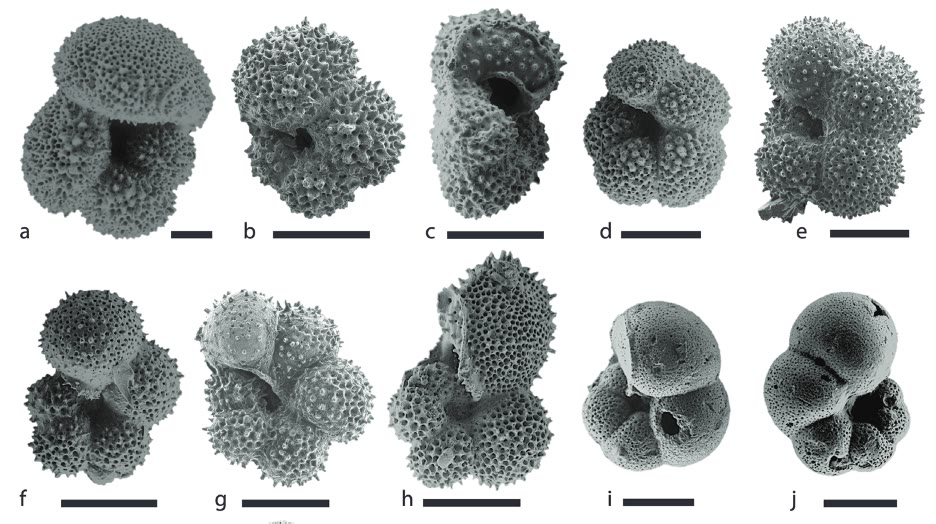
\includegraphics[width=0.62\linewidth]{images/book2/g12-planktic-foraminifera.jpg}

{\small Conchas de dez espécies de foraminíferos que viviam flutuando no
oceano, vistas com um microscópio eletrônico de varredura; cada barra de
escala mede \qty{150}{\micro\metre}, então cada concha tem mais ou menos o
tamanho de um grão de areia. Marci Robinson, USGS (domínio público, via
Wikimedia Commons).}
\end{omfigure}
% ledger: photo:g12-forams

O oxigênio de uma concha vem da água do mar. A água feita com o isótopo leve
oxigênio-16 evapora mais facilmente, e a neve que forma os mantos de gelo é
por isso pobre em oxigênio-18. Quando os mantos de gelo crescem, eles
armazenam essa água leve, e o oceano que fica se torna mais rico em
oxigênio-18; o mesmo acontece com as conchas que crescem nele, tanto mais
quanto mais fria é a água. A parte de oxigênio-18 nas conchas dos
foraminíferos do fundo do mar, escrita
$\delta^{18}\mathrm{O}$ e dada em partes por mil, é assim um \omterm{def:g12:past-climates:proxy}{indicador} do
volume de gelo sobre os continentes e da temperatura do \omterm{def:g10:layered-ocean:thermocline}{oceano profundo}:
quanto mais alta, mais gelo e mais fria a água.
% ledger: nasaeo:o18, lr04:stack

O registro abaixo, chamado LR04, empilha as medições de 57 testemunhos de
todos os oceanos numa só curva de 5.3 milhões de anos.

\begin{omfigure}
\begin{tikzpicture}
\begin{axis}[omrecord, scale only axis, width=0.86\linewidth, height=4.8cm,
  xmin=0, xmax=5.32, x dir=reverse, ymin=2.4, ymax=5.3, y dir=reverse,
  xtick={0,0.5,...,5}, ytick={2.5,3,...,5},
  x tick label style={/pgf/number format/.cd, fixed, precision=1},
  y tick label style={/pgf/number format/.cd, fixed, fixed zerofill, precision=1},
  xlabel={milhões de anos antes de 1950},
  ylabel={$\delta^{18}\mathrm{O}$ das conchas (\unit{\permil})}]
\fill[omProp!14] (axis cs:1.25,2.4) rectangle (axis cs:0.7,5.3);
% data:lr04 (the stack only; ice_age_records.py)
\addplot[omDef!85!black, line width=0.35pt] table[x=age_Ma, y=d18O] {figdata/out/grade-12-ice_age_records-lr04.dat};
\addplot[omThm, line width=1pt, densely dashed, unbounded coords=jump] table[x=age_Ma, y=d18O] {figdata/out/grade-12-ice_age_records-lr04mean.dat};
\coordinate (mpt) at (axis cs:0.975,2.45);
\coordinate (mm) at (axis cs:5.22,4.92);
\coordinate (arr) at (axis cs:5.12,3.9);
\end{axis}
\node[font=\scriptsize, anchor=north, align=center] at (mpt) {de 41 000 a\\100 000 anos};
\draw[omThm, line width=1pt, densely dashed] (mm) -- ($(mm)+(0.5,0)$) node[right, font=\scriptsize, text=omThm] {médias de 5.3 a 3 e de 1 a 0 milhão de anos atrás};
\draw[-{Stealth}, black!70] (arr) -- ++(0,-0.9) node[midway, right, font=\scriptsize, align=left] {mais gelo,\\mais frio};
\end{tikzpicture}

{\small Cinco milhões de anos do \omterm{def:g10:layered-ocean:thermocline}{oceano profundo} nas conchas dos
foraminíferos do fundo do mar; o eixo vertical está invertido, para que as
épocas frias e cobertas de gelo fiquem embaixo. As retas tracejadas são as
médias da primeira e da última partes. Sombreado: a passagem de um ritmo de
\num{41000} anos a um ritmo de cerca de \num{100000} anos. Dados: Lisiecki e
Raymo (2005), o empilhamento LR04.}
\end{omfigure}
% ledger: data:lr04, lr04:stack, clark06:mpt

Lido com o método acima, o registro diz três coisas.
\begin{itemize}
  \item \emph{A Terra esfriou e o seu gelo cresceu.} O valor médio sobe de
        \qty{3.03}{\permil} entre 5.3 e 3 milhões de anos atrás para
        \qty{4.15}{\permil} no último milhão de anos.
  \item \emph{As oscilações aumentaram.} Épocas glaciais e \omterm{def:g12:past-climates:glacial-cycle}{interglaciais} se
        alternam ao longo de todo o registro, mas oscilam cada vez mais: no
        \omterm{def:g12:past-climates:lgm}{Último Máximo Glacial}, o valor era de \qty{4.92}{\permil}, contra
        \qty{3.23}{\permil} hoje.
  \item \emph{O ritmo mudou.} Entre 2.6 e 1.3 milhões de anos atrás, o
        período mais forte do registro, calculado a partir dos seus dados, é
        de \num{41000} anos; nos últimos \num{700000} anos, é de cerca de
        \num{98000} anos, o ritmo dos \omterm{def:g12:past-climates:ice-core}{testemunhos de gelo}. A mudança
        aconteceu entre cerca de 1.25 e 0.7 milhão de anos atrás.
\end{itemize}
% ledger: data:lr04, clark06:mpt (ice_age_records.py: lr04_mean_3_5Ma 3.032, lr04_mean_0_1Ma 4.147, lr04_lgm 4.92, lr04_today 3.23, periods 41.0 and 98.5 kyr)

Esses períodos não são obra do acaso. Em 1976, James Hays, John Imbrie e
Nicholas Shackleton encontraram nos sedimentos dos oceanos austrais três
ritmos, de \num{23000}, \num{42000} e cerca de \num{100000} anos, que são os
períodos das lentas mudanças da órbita e do eixo da Terra: a precessão do
eixo, a inclinação do eixo (cerca de \num{41000} anos) e a forma da órbita
(cerca de \num{100000} anos). Essas mudanças deslocam a luz do Sol que cada
latitude recebe em cada estação, e elas marcam o compasso dos \omterm{def:g12:past-climates:glacial-cycle}{ciclos
glaciais}. Como elas o fazem, e por que o lento ritmo de \num{100000} anos
passou a dominar, é assunto de um curso universitário.
% ledger: hays76:periods, nasa:milankovitch, lr04:stack, clark06:mpt

\begin{dated}{2025}
Em janeiro de 2025, o projeto Beyond EPICA anunciou que um testemunho
perfurado em Little Dome~C, a cerca de \qty{35}{km} da estação Concordia, em
Dome~C, contém um registro contínuo de cerca de 1.2 milhão de anos nos seus
\qty{2480}{m} superiores. Ele cobre a época
em que o ritmo glacial passou de \num{41000} a \num{100000} anos, e o gelo e
o seu ar estão sendo analisados.
\end{dated}
% ledger: ku25:beyond-epica, ipev25:little-dome-c

\section{Os climas do tempo profundo}

Mais atrás que os \omterm{def:g12:past-climates:ice-core}{testemunhos de gelo}, os climas do passado são lidos nos
sedimentos, nas folhas e nos solos fósseis, e nos isótopos. O IPCC escolheu
alguns \emph{períodos de referência}, bem estudados, cujos climas ajudam a
julgar as mudanças de hoje e de amanhã. O gráfico abaixo dá a sua
temperatura global da superfície, em relação a 1850--1900.

\begin{omfigure}
\begin{tikzpicture}
\begin{axis}[omrecord, width=0.86\linewidth, height=5.4cm, xmin=-9, xmax=27,
  ymin=0.4, ymax=6.6, y dir=reverse, ytick={1,...,6}, ymajorgrids=false,
  yticklabels={{PETM, 56 Ma}, {EECO, 53--49 Ma}, {MPWP, 3.3--3.0 Ma},
    {LIG, 129--116 ka}, {LGM, 23--19 ka}, {MH, 6.5--5.5 ka}},
  y tick label style={font=\scriptsize},
  xlabel={temperatura em relação a 1850--1900 (\unit{\degreeCelsius})}]
% ipcc:fig2-34 (DEEP in ice_age_records.py)
\addplot[draw=none, mark=none, restrict expr to domain={\thisrow{tlo}}{0:30},
  error bars/.cd, x dir=both, x explicit,
  error bar style={line width=5pt, omWarm!75}, error mark=none]
  table[x expr={(\thisrow{tlo}+\thisrow{thi})/2}, y=idx,
        x error expr={(\thisrow{thi}-\thisrow{tlo})/2}] {figdata/out/grade-12-ice_age_records-deep.dat};
\addplot[draw=none, mark=none, restrict expr to domain={\thisrow{tlo}}{-30:-0.01},
  error bars/.cd, x dir=both, x explicit,
  error bar style={line width=5pt, omCold!75}, error mark=none]
  table[x expr={(\thisrow{tlo}+\thisrow{thi})/2}, y=idx,
        x error expr={(\thisrow{thi}-\thisrow{tlo})/2}] {figdata/out/grade-12-ice_age_records-deep.dat};
\draw[black!60] (axis cs:0,0.4) -- (axis cs:0,6.6);
\draw[omThm, densely dashed, line width=0.8pt] (axis cs:1.09,0.4) -- (axis cs:1.09,6.6);
\node[font=\scriptsize, text=omThm, anchor=west, fill=white, inner sep=1pt] at (axis cs:1.6,4.55) {2011--2020};
\end{axis}
\end{tikzpicture}

{\small Temperatura global da superfície de seis períodos de referência do
passado, faixas muito prováveis, em relação a 1850--1900; tracejada: a
década 2011--2020. Siglas em inglês: PETM, Máximo Térmico do
Paleoceno--Eoceno; EECO, Ótimo Climático do Eoceno Inferior; MPWP, Período
Quente do Plioceno Médio; LIG, Último Interglacial; LGM, \omterm{def:g12:past-climates:lgm}{Último Máximo
Glacial}, o único frio (em azul); MH,
Holoceno Médio. Valores: IPCC AR6 WG1, Figura 2.34.}
\end{omfigure}
% ledger: ipcc:fig2-34, ipcc:gsat-2011-2020, ipcc:ref-periods

\begin{center}
\small
\begin{tabular}{|l|c|c|c|}
\hline
\textbf{período} & \textbf{temperatura (\unit{\degreeCelsius})} & \textbf{gás carbônico (ppm)} & \textbf{nível do mar (m)} \\
\hline
PETM, 56 Ma & de $+10$ a $+25$ & cerca de 900, subindo a 2000 & --- \\
EECO, 53--49 Ma & de $+10$ a $+18$ & de 1150 a 2500 & de $+70$ a $+76$ \\
MPWP, 3.3--3.0 Ma & de $+2.5$ a $+4.0$ & de 360 a 420 & de $+5$ a $+25$ \\
LIG, 129--116 ka & de $+0.5$ a $+1.5$ & de 266 a 282 & de $+5$ a $+10$ \\
\textcolor{omCold}{LGM, 23--19 ka} & \textcolor{omCold}{de $-7$ a $-5$} & \textcolor{omCold}{de 188 a 194} & \textcolor{omCold}{de $-134$ a $-125$} \\
MH, 6.5--5.5 ka & de $+0.2$ a $+1.0$ & de 260 a 268 & de $-3.5$ a $+0.5$ \\
\hline
\end{tabular}

\medskip
{\small Os períodos de referência: temperatura global da superfície em
relação a 1850--1900, gás carbônico e nível global do mar em relação a 1900.
IPCC AR6 WG1, Figura 2.34.}
\end{center}
% ledger: ipcc:fig2-34

O Máximo Térmico do Paleoceno--Eoceno foi um aquecimento brusco, quando um
grande pulso de carbono chegou ao oceano e ao ar: o oceano ficou mais ácido
e mais pobre em oxigênio, e muitas espécies do mar profundo se extinguiram.
No Ótimo Climático do Eoceno Inferior, o gás carbônico ficou acima de
\qty{1000}{ppm} durante milhões de anos, não havia gelo polar, e florestas
quase tropicais cresciam a \ang{70}~Sul. O Período Quente do Plioceno Médio
é a última vez em que o gás carbônico esteve perto do de hoje: o Ártico era
muito mais quente que agora, e o mar estava mais alto. No Último
Interglacial, os mantos de gelo da Groenlândia e da Antártida Ocidental eram
menores e o mar mais alto que hoje, e hipopótamos viviam na Grã-Bretanha.
% ledger: ipcc:ref-periods, ipcc:fig2-34, ipcc:mpwp-eeco

Esses arquivos põem o presente em perspectiva, e o próprio IPCC faz a
comparação. Em 2019, o gás carbônico do ar era mais alto do que em qualquer
momento dos últimos dois milhões de anos, pelo menos (\emph{alta
confiança}), e os aumentos do gás carbônico e do metano desde 1750 superam
de longe as variações naturais entre \omterm{def:g12:past-climates:glacial-cycle}{períodos glaciais} e \omterm{def:g12:past-climates:glacial-cycle}{interglaciais} ao
longo de pelo menos \num{800000} anos (\emph{muito alta confiança}). A
temperatura global da superfície subiu mais depressa desde 1970 do que em
qualquer outro período de 50 anos ao longo de pelo menos os últimos
\num{2000} anos (\emph{alta confiança}). A década 2011--2020 foi mais quente
que os séculos mais quentes do \omterm{def:g12:past-climates:glacial-cycle}{interglacial} atual, há cerca de \num{6500}
anos, e próxima do calor do Último Interglacial, há cerca de \num{125000}
anos (\emph{média confiança}).
% ledger: ipcc:co2-ch4-800kyr, ipcc:fastest-2000yr, ipcc:co2-2myr

A velocidade da mudança também pode ser comparada. De 1970 a 2025, a
tendência do registro da temperatura global é de \qty{0.20}{\degreeCelsius}
por década, ou cerca de \qty{20}{\degreeCelsius} por mil anos se fosse
mantida; o aquecimento ao sair do último \omterm{def:g12:past-climates:glacial-cycle}{período glacial} foi em média de
cerca de \qty{0.86}{\degreeCelsius} por mil anos. As causas da mudança de
hoje, e o que ela pode vir a ser, são o assunto do \cref{ch:g12:climate-change}.
% ledger: data:gistemp (ice_age_records.py: rate_1970_2025_C_per_decade 0.2012), ipcc:lgm-cooling, ipcc:ref-periods

\section{Exercícios}

\begin{exercise}[$\star$]\label{exo:g12:past-climates:1}
Dê o termo: (a) uma grandeza medida num arquivo que substitui uma variável
climática não medida; (b) um cilindro de gelo extraído por perfuração de um
manto de gelo; (c) um intervalo quente entre dois \omterm{def:g12:past-climates:glacial-cycle}{períodos glaciais}; (d) a
leitura da vegetação do passado a partir do pólen fóssil; (e) a época, de
cerca de \num{23000} a \num{19000} anos atrás, em que os últimos mantos de
gelo estavam no seu maior tamanho.
\end{exercise}

\begin{exercise}[$\star$]\label{exo:g12:past-climates:2}
Para cada \omterm{def:g12:past-climates:proxy}{indicador}, dê o seu arquivo e aquilo sobre o que ele informa: (a)
o ar das bolhas; (b) a parte de pólen de carvalho; (c) o oxigênio-18 das
conchas dos foraminíferos do fundo do mar; (d) a largura dos anéis das
árvores.
\end{exercise}

\begin{exercise}[$\star$]\label{exo:g12:past-climates:3}
Durante a última transição deglacial, de cerca de \num{18000} a \num{11000}
anos atrás, o nível do mar subiu de cerca de \qty{-120}{m} a \qty{-50}{m}.
(a) Calcule a taxa média de subida, em milímetros por ano. (b) De 2006 a
2018, o nível do mar subiu \qty{3.7}{mm} por ano. Compare.
\end{exercise}

\begin{exercise}[$\star$]\label{exo:g12:past-climates:4}
A temperatura global subiu \qty{0.20}{\degreeCelsius} por década de 1970 a
2025. Exprima essa taxa por século e por mil anos.
\end{exercise}

\begin{exercise}[$\star$]\label{exo:g12:past-climates:5}
Hays, Imbrie e Shackleton encontraram três ritmos nos sedimentos oceânicos:
\num{23000}, \num{42000} e cerca de \num{100000} anos. (a) Associe cada um à
precessão do eixo, à inclinação do eixo e à forma da órbita.
(b) Quantos ciclos de \num{41000} anos cabem em \num{1000000} anos? Quantos
ciclos de \num{100000} anos?
\end{exercise}

\begin{exercise}[$\star\star$]\label{exo:g12:past-climates:6}
A reta de mínimos quadrados do capítulo é $\mathrm{CO_2} \approx 266.6 +
7.83\,\Delta T$ (ppm, com $\Delta T$ em \unit{\degreeCelsius}).
(a) Preveja o gás carbônico para a temperatura média do \omterm{def:g12:past-climates:lgm}{Último Máximo
Glacial} em Dome~C, \qty{-9.4}{\degreeCelsius}, e compare com os
\qty{190}{ppm} medidos. (b) Preveja-o para o ponto mais quente,
\qty{+5.5}{\degreeCelsius}, e compare com o valor mais alto medido,
\qty{299}{ppm}. (c) Use a reta para estimar a temperatura em Dome~C que
corresponderia a \qty{427}{ppm}, o valor de 2025 em Mauna Loa. Por que este
último uso da reta não se justifica?
\end{exercise}

\begin{exercise}[$\star\star$]\label{exo:g12:past-climates:7}
Use o \omterm{def:g12:past-climates:pollen}{diagrama polínico} do lago das Colinas de Varden. (a) Qual é o pólen
dominante a \qty{580}{cm}, e que paisagem ele indica? (b) A mesma pergunta a
\qty{340}{cm}. (c) Que árvore se espalha primeiro depois do frio, e que
árvores chegam por último? (d) Por que a chegada de uma árvore poderia se
atrasar em relação ao aquecimento que a permitiu?
\end{exercise}

\begin{exercise}[$\star\star$]\label{exo:g12:past-climates:8}
No mesmo testemunho, a lama a \qty{600}{cm} tem \num{14000} anos e a de
\qty{300}{cm} \num{6000} anos, com uma taxa de deposição constante.
(a) Calcule essa taxa em milímetros por ano. (b) Encontre a idade do limite
entre as zonas 2 e 3, a \qty{470}{cm}. (c) Quantos anos representa uma
fatia de \qty{1}{cm} de espessura?
\end{exercise}

\begin{exercise}[$\star\star$]\label{exo:g12:past-climates:9}
No mapa do Sudeste Asiático, as terras acima do mar passam de 4.11 a
7.16 milhões de quilômetros quadrados quando o mar baixa \qty{130}{m}.
(a) Calcule o ganho e a sua porcentagem. (b) No mapa, uma descida de cerca
de \qty{36}{m} basta para ligar Bornéu à Ásia. A ilha esteve ligada durante
todo o \omterm{def:g12:past-climates:lgm}{Último Máximo Glacial}? Explique. (c) Por que a linha de costa do mapa
é só aproximada?
\end{exercise}

\begin{exercise}[$\star\star$]\label{exo:g12:past-climates:10}
No registro LR04, o valor no \omterm{def:g12:past-climates:lgm}{Último Máximo Glacial} é de
\qty{4.92}{\permil}, e o de hoje, \qty{3.23}{\permil}. (a) Qual é o mais
alto, e é isso que você esperava? Explique com os mantos de gelo. (b) Por
que o eixo vertical do registro é traçado invertido?
\end{exercise}

\begin{exercise}[$\star\star$]\label{exo:g12:past-climates:11}
Um amigo diz: ``A correlação de 0.92 entre a temperatura antártica e o gás
carbônico prova que o gás carbônico controlou as glaciações.'' (a) O que
uma correlação mostra, e o que ela não mostra? (b) Dê duas outras
explicações que dariam a mesma correlação. (c) Que tipo de informação sobre
os dois registros ajudaria a decidir?
\end{exercise}

\begin{exercise}[$\star\star\star$]\label{exo:g12:past-climates:12}
O período mais forte do registro LR04 é de \num{41000} anos entre 2.6 e 1.3
milhões de anos atrás, e de \num{98500} anos nos últimos \num{700000} anos.
(a) Quantos ciclos cabem em cada janela? (b) Que mudança da órbita ou do
eixo da Terra corresponde a cada período? (c) Explique por que um registro
com uma amostra a cada \num{2000} anos pode mostrar esses ritmos, mas não
uma mudança que durou um século.
\end{exercise}

\begin{exercise}[$\star\star\star$]\label{exo:g12:past-climates:13}
A taxa de aumento do gás carbônico foi de 192 a \qty{198}{ppm} por século em
1995--2014. Durante o Máximo Térmico do Paleoceno--Eoceno, ela foi de 4 a
\qty{42}{ppm} por século, e durante a última transição deglacial, no máximo
cerca de \qty{10}{ppm} por século. (a) Quantas vezes mais rápido foi o
aumento recente que o aumento mais rápido da última deglaciação? (b) E que
a estimativa mais lenta e a mais rápida do PETM? (c) O aumento do PETM foi
de cerca de 900 a cerca de \qty{2000}{ppm}. Quanto tempo ele teria levado a
\qty{42}{ppm} por século, e à taxa de hoje?
\end{exercise}

\begin{exercise}[$\star\star\star$]\label{exo:g12:past-climates:14}
O IPCC estima que a temperatura global subiu de 1 a
\qty{1.5}{\degreeCelsius} por mil anos na parte mais rápida da última
deglaciação, e que sobre a Groenlândia ela subiu cerca de dez vezes mais
depressa nos séculos de aquecimento mais rápido. (a) Dê a taxa da
Groenlândia em \unit{\degreeCelsius} por mil anos e por década. (b) Compare-a
com a taxa global de hoje, de \qty{0.20}{\degreeCelsius} por década. (c) Por
que uma taxa local não deve ser comparada diretamente com uma taxa global?
\end{exercise}

\begin{exercise}[$\star\star\star$]\label{exo:g12:past-climates:15}
O nível do mar estava a cerca de \qty{-50}{m} há \num{11000} anos; suponha
que ele tenha subido então a uma taxa constante de \qty{12}{m} por mil anos,
a taxa média da deglaciação principal. (a) Quando ele passou de
\qty{-36}{m}, o nível que liga Bornéu à Ásia no mapa? (b) Depois dessa
época, uma pessoa poderia ir a pé de Bornéu até a Península Malaia? (c)
Quanto tempo o mar levaria para subir os últimos \qty{36}{m}, se tivesse
continuado na mesma velocidade?
\end{exercise}

\begin{problem}[{Problema de fim de semana --- 800 000 anos de gelo antártico}]
\label{pb:g12:past-climates:1}
% ledger: data:edc-jouzel, data:co2-bereiter, data:lr04, data:gistemp, ipcc:lgm-cooling, ipcc:ref-periods, hays76:periods, clark06:mpt
% values (ice_age_records.py): edc -10.58 / +5.46, co2 173.71 / 298.6, r 0.9165, fit 266.57 + 7.827 T,
% LGM -9.389 / 189.67, 11-9 ka -0.360 / 264.10, period 97.5, rate 0.2012 per decade, ratio 23.48
O gelo de Dome~C e o ar das suas bolhas dão os valores seguintes. A
temperatura é a variação sobre o gelo em relação aos últimos mil anos.

\begin{center}
\small
\begin{tabular}{|l|c|c|}
\hline
 & \textbf{variação de temperatura (\unit{\degreeCelsius})} & \textbf{gás carbônico (ppm)} \\
\hline
mais frio, há uns \num{24000} anos & $-10.6$ & --- \\
mais quente, há uns \num{129000} anos & $+5.5$ & --- \\
gás carbônico mínimo e máximo & --- & 174 e 299 \\
média de \num{23000} a \num{19000} anos atrás & $-9.4$ & 190 \\
média de \num{11000} a \num{9000} anos atrás & $-0.4$ & 264 \\
\hline
\end{tabular}
\end{center}

O período mais forte do registro de temperatura é de cerca de \num{98000}
anos, e os 1639 pares de valores dão um coeficiente de correlação de 0.92.

\medskip
\noindent\textbf{Parte I --- Ler os dois registros.}
\begin{enumerate}
  \item Que parte do gelo registra a temperatura, e qual registra o gás
        carbônico?
  \item Calcule a amplitude total da variação de temperatura em Dome~C.
  \item Calcule a amplitude total do gás carbônico.
  \item O que um coeficiente de correlação de 0.92 diz sobre os dois
        registros?
  \item Na figura do capítulo com o eixo do tempo, hoje está à direita. Por
        que é preciso verificar em que sentido o tempo corre antes de ler uma
        figura assim?
\end{enumerate}

\medskip
\noindent\textbf{Parte II --- Valores glaciais e interglaciais.}
\begin{enumerate}[resume]
  \item Defina um \omterm{def:g12:past-climates:glacial-cycle}{período glacial} e um \omterm{def:g12:past-climates:glacial-cycle}{interglacial}.
  \item Em qual dos dois nós vivemos, e desde quando?
  \item Quantos ciclos de \num{98000} anos cabem em \num{800000} anos?
  \item Que mudança da órbita da Terra tem um período próximo de
        \num{100000} anos?
  \item Antes de cerca de 1.25 milhão de anos atrás, qual era o ritmo
        principal dos \omterm{def:g12:past-climates:glacial-cycle}{ciclos glaciais}?
\end{enumerate}

\medskip
\noindent\textbf{Parte III --- A última deglaciação.}
\begin{enumerate}[resume]
  \item Quanto subiu a temperatura sobre Dome~C entre o \omterm{def:g12:past-climates:lgm}{Último Máximo
        Glacial} e o intervalo de \num{11000} a \num{9000} anos atrás?
  \item Quanto subiu o gás carbônico no mesmo intervalo?
  \item A temperatura global do \omterm{def:g12:past-climates:lgm}{Último Máximo Glacial} era de 5 a
        \qty{7}{\degreeCelsius} mais baixa que a de 1850--1900. Tome o meio
        dessa faixa. A variação antártica é maior ou menor?
  \item A última transição deglacial durou de \num{18000} a
        \num{11000} anos atrás. Quanto tempo é isso?
  \item Calcule a taxa média de aquecimento global durante a transição, em
        \unit{\degreeCelsius} por mil anos.
  \item Exprima essa taxa em \unit{\degreeCelsius} por década.
\end{enumerate}

\medskip
\noindent\textbf{Parte IV --- A taxa de hoje em comparação.}
\begin{enumerate}[resume]
  \item De 1970 a 2025, a temperatura global subiu
        \qty{0.20}{\degreeCelsius} por década. Exprima essa taxa por mil
        anos.
  \item Quantas vezes mais rápido é o aquecimento de hoje que o aquecimento
        médio da última deglaciação?
  \item Na parte mais rápida da deglaciação, a temperatura global subiu
        de 1 a \qty{1.5}{\degreeCelsius} por mil anos. Quantas vezes mais
        rápida que essas é a taxa de hoje?
  \item Conclua: quantas vezes mais rápido que o aquecimento ao sair da
        última glaciação é o aquecimento global de hoje?
\end{enumerate}
\end{problem}
